\documentclass[a4paper]{article}
\usepackage{xeCJK}
\usepackage{verbatim}
\usepackage{graphicx}
\usepackage{hyperref}
\hypersetup{colorlinks}
%\setCJKmainfont{Noto Sans CJK SC}
\setCJKmainfont{宋体}
\setCJKmonofont{微软雅黑}
\pagestyle{plain}
\begin{document}
	\section*{Info}
		\begin{tabular}{ll}
  Name: & 周明东 \\
  Tel: & 13922835173 \\
  E-mail: & mingdong\_zhou\_gxbs@sina.com \\
  GitHub: & https://github.com/catRat
\end{tabular}

	\section*{Skills}
		\begin{itemize}
\item 熟练使用 Window 操作系统, 了解 Linux 操作系统.
\item 熟练使用 Excel, 包括 Excel 的常用函数, Excel 的数据透视表.
\item 熟练使用 Word.
\item 熟练使用 PowerPoint.
\item 熟练使用 R, SPSS, Python.
\item 熟练使用 R 进行数据的清理, 包括
\begin{itemize}
\item 长格式与宽格式的转化,
\item 日期值处理,
\item 字符数据处理,
\end{itemize}
\item 熟练使用 R 的 ggplot2 完成数据可视化工作.
\item 熟练使用 SQL 语言.
\item 熟练使用 R 完成假设检验, 差异分析, 回归分析.
\item 了解 Shiny Server, 能够搭建 Shiny Server.
\end{itemize}

	\section*{Education Experience}
		\section{教育经历}
\begin{itemize}
	\item 2013-2017年,就读于河池学院数学与统计学院,专业是统计学。我没有在2017年修够学分,也没有再可延期的时间里修完学分,所以我没有从学校中毕业,是个结业生。%也并非什么大病,它是过敏性的鼻炎,还有轻微胃病。
	\item 2012-2013年,补习于我在广西百色市祈福高级中学。
	\item 2009-2012年,就读于广西百色市百色民族高级中学,曾任物理科代表。
	\item 2007-2009年,就读于广西那坡县那坡民族初级中学,曾任学习委员,班长。
	\item 2005-2007年,就读于广西那坡县百合乡百合中学,曾任领操员。
	\item 1999-2005年,就读于广西那坡县百合乡那乐村那乐小学。
\end{itemize}

	\section*{Work Experience}
		\section{工作经历}
\begin{itemize}
	\item 2017年-2018年10月。深圳鸿安货运代理有限公司数据文员,是我的第一份工作。深圳鸿安货运代理有限公司是一家从事物流服务(进出口)的公司。我的工作内容由两部分组合,第一部分是使用一个文件对一个系统进行数据更新,每天更新一次,这份文件是包含航线,船东,货物,价格关系的表,第二部分是为和我同属一个航线的同事提供一个report,report的主要部分是几个透视表,我会在Outlook里发给他们。在大部分时间里,我都在和Excel打交道。
	\item 2018年11月-2019年6月。深圳裕展精密科技有限公司生产员,是我的第二份工作。
\end{itemize}

	\section*{Present}
		我目前还在公司的岗位中, 公司的岗位交接需要 1 个月的时间. 现在的我积极考虑换工作. 

	\section*{Code Show}
		利用 R 的数据结构和工具, 我能够高效地完成往往需要 VBA 才能完成的工作. 以下为为了完成某一数据处理工作而写的 R 脚本, 欢迎阅读. 我也可以写 Pyhont 脚本, 之所以不写, 是因为如果一个工具能够很好地完成某种任务, 为什么还要考虑其他工具.
		\verbatiminput{GetCode.R}	
		\verbatiminput{GetId.R}	
		\verbatiminput{Select.R}
		\verbatiminput{blackcat.R}	
	\section*{Graph Show}
		\begin{figure}
		\begin{center}
		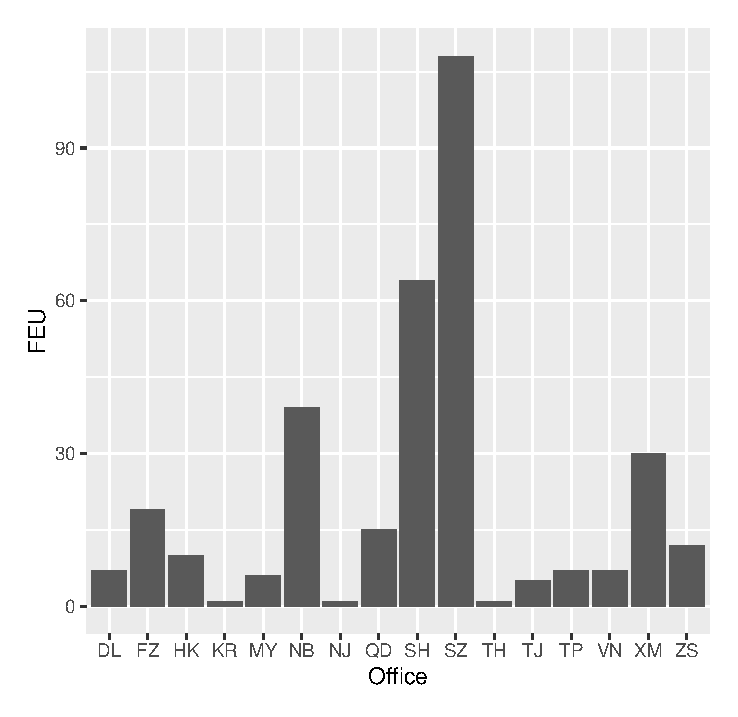
\includegraphics{Rplot01}
		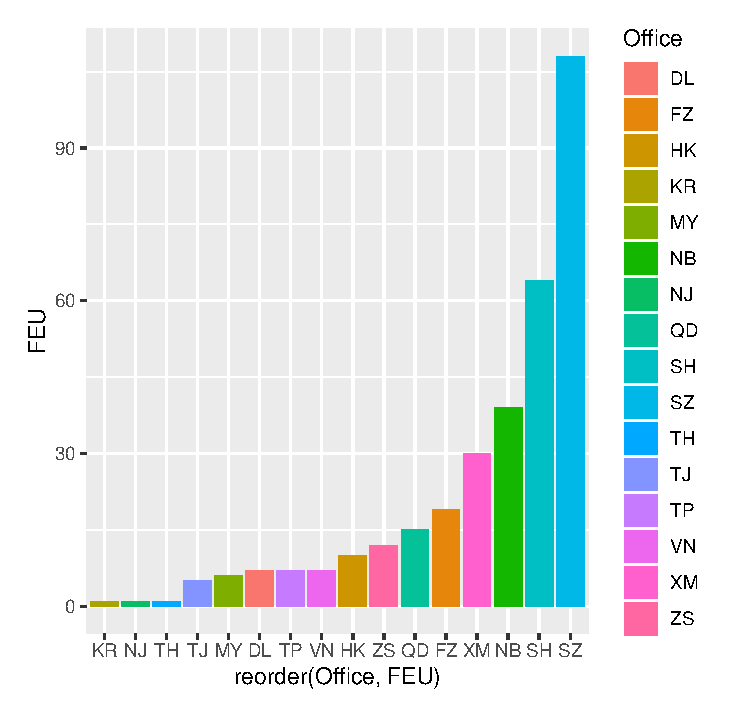
\includegraphics{Rplot03}
		\end{center}
		\end{figure}
		\begin{figure}
		\begin{center}
		\includegraphics{Rplot04}
		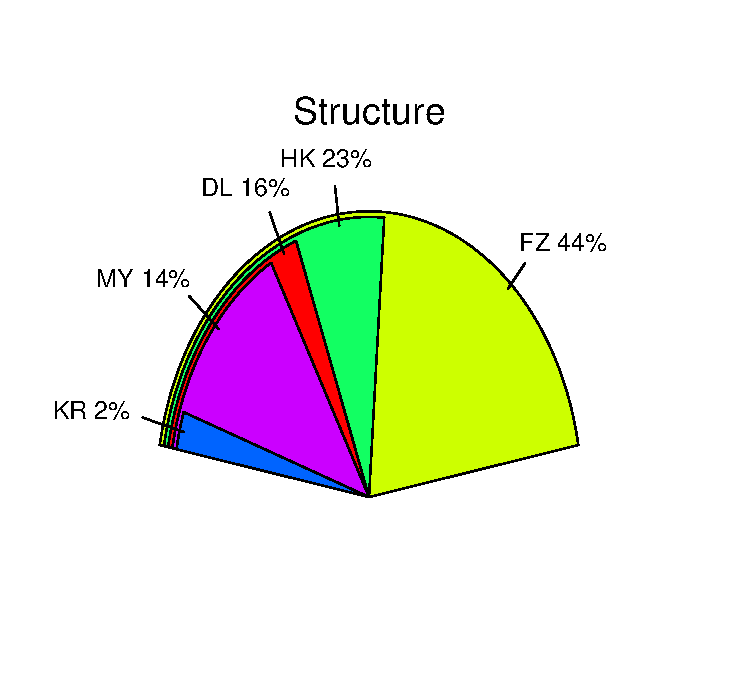
\includegraphics{Rplot09}
		\end{center}
		\end{figure}
\end{document}
